%
%
%

\chapter{Conversion to Discrete Time: Tustin's Method}

\section{Problem Statement and Learning Objectives}

The student will be able to:
\begin{itemize}
    \item Explain how the Nyquist sampling rate applies to discrete  time controllers and
    how to apply it to select a sampling rate.
    \item Use Tustin's method by hand to convert a continuous-time/frequency-domain controller
    to discrete time.
    \item Use Tustin's method in the computer to covert a transfer function to discrete time.
    \item Convert a discrete time transfer function, using the inverse $Z$ transform, to
    a difference equation.
    \item  Program a loop in pseudo-code which can implement the designed discrete time controller.
\end{itemize}

%%%%** Section 1
\section{Overview}
Tustin's method (aka \href{https://en.wikipedia.org/wiki/Bilinear_transform}{the Bilinear Transform}) lets us convert a controller designed in the continuous time
LaPlace domain to an equivalent (over a certain bandwidth) discrete time
controller.  In order to implement a controller in a digital platform such as a
microcontroller or FPGA, we must have it expressed in discrete time.

In this chapter, we will describe a procedure to convert a continuous time transfer function (such as a controller you might design on  the  computer) into a line of code you could build into a software application. 	%<*h>

In the following, it will help if you have been exposed to some discrete time signals and systems theory (the Z-Transform), but full knowledge of Z-transforms is not required to calculate this conversion.
Our procedure will boil down to the following process for converting your continous time controller
into computer code.

\begin{enumerate}
  \item Model your system
  \item Design your controller as in previous chapters.
  \item Convert controller from continuous time to discrete time
  \item Convert your discrete time controller to a digital filter which can be easily coded.
  \item Code and test your filter in the computer.
\end{enumerate}

%\end{frame}
%%%%** Section 2
\section{Discrete Time and Z transform review/intro}
%\begin{frame}

\begin{figure}[h]
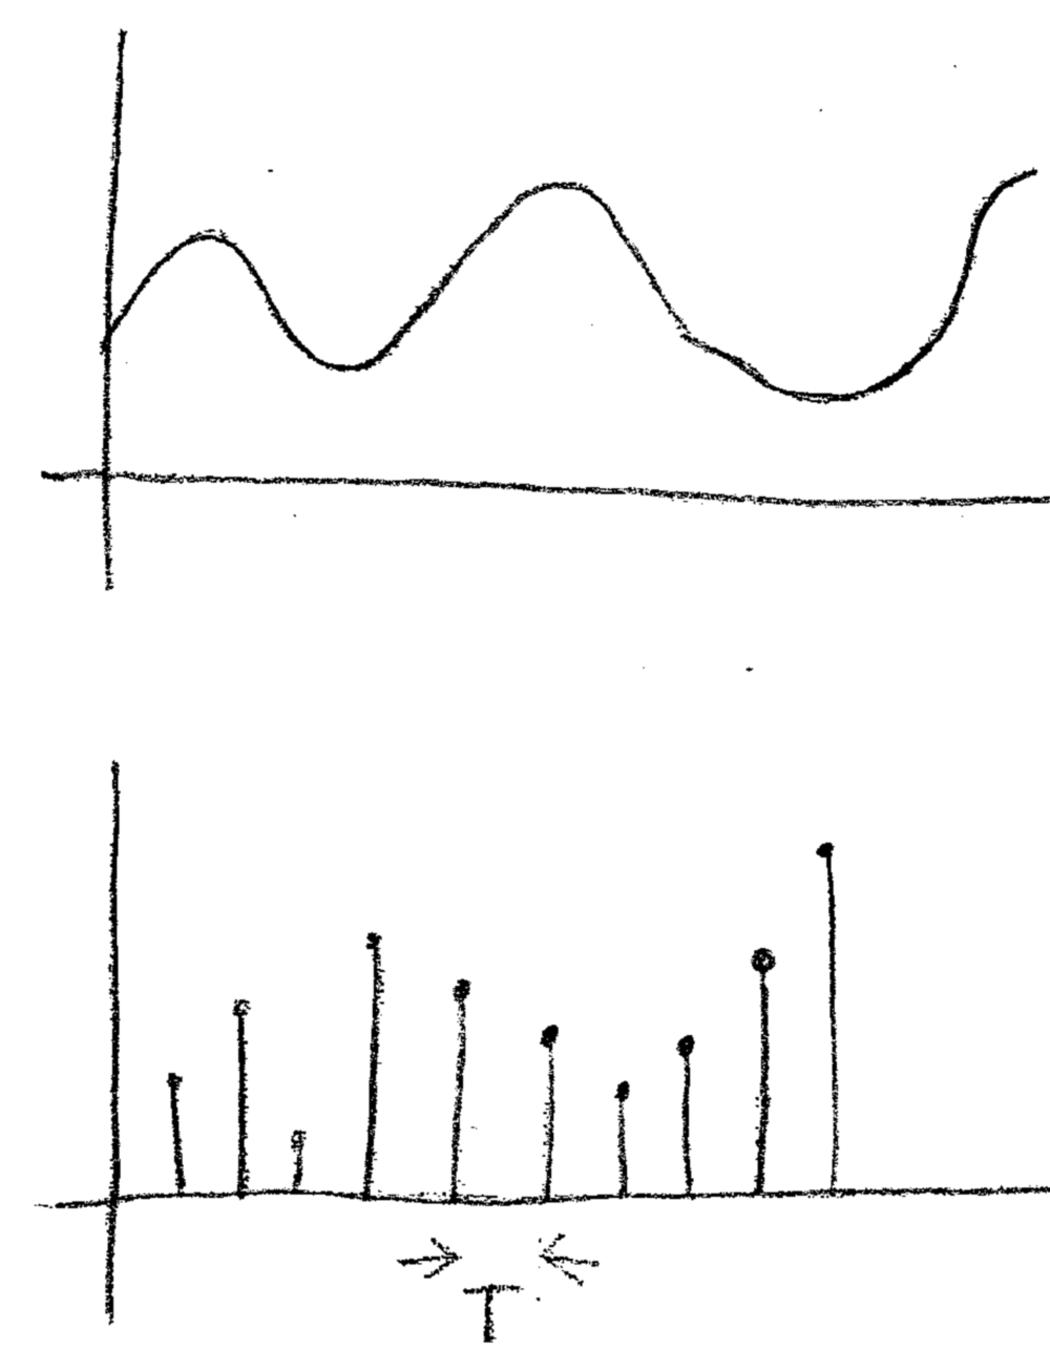
\includegraphics[width=3.5in]{figs11/cont_disc_sigsa.png}	%<h>
%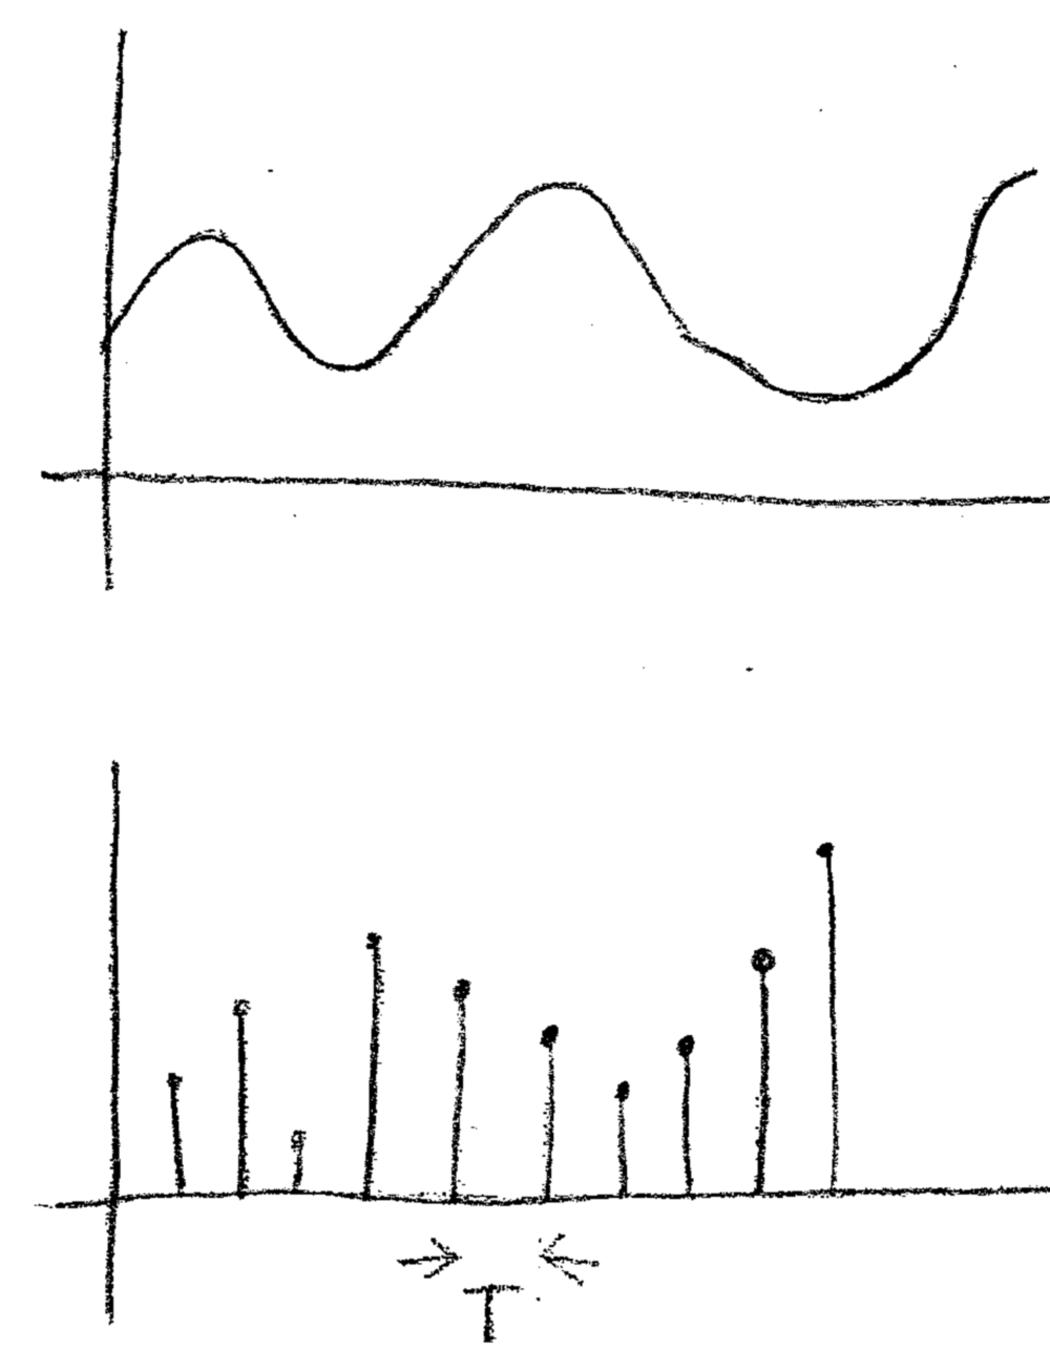
\includegraphics[width=2.5in]{figs11/cont_disc_sigsa.png}
\caption{Continuous time (top) and discrete time (bottom) signals. The time between samples is $T$.}\label{FigContinuousDiscreteSignals}
\end{figure}

%\end{frame}
%\begin{frame}

A discrete time signal, also known as a ``sampled data signal'', is a series of unit impulses,
at regular times $t=nT, n=\{0,1,2,3,....\}$,
scaled by the signal values at each sample time (Figure \ref{FigContinuousDiscreteSignals}).
If there is a continuous signal, $x(t)$, the discrete time version of that signal is
\[
x(n) = \sum_n \delta(t-nT)\times x(nT)  \qquad \qquad n = 0,1,2 \dots
\]

The unilateral Z-Transform (a discrete time analog of the Laplace Transform) is
\[
X(z) = \sum_{n=0}^{n=\infty} x(n)z^{-n}
\]
where $z$ is a complex number (like $s$), usually represented $Ae^{j\psi}$.

The Z-Transform can be used like the Laplace transform to analyze systems expressed as digital filters.


%\end{frame}
%%%%** Section 2.1
\subsection{Discrete and Continuous Comparison Table}
%\begin{frame}

In the following table, we list the analogous concepts between discrete time and continuous time.

\renewcommand\arraystretch{1.75}% Vertical Row size, 1.0 is for standard spacing)
\begin{centering}
\begin{tabular}{c|c}
{\bf Sampled World  }         &  {\bf Continuous World  }   \\ \hline
$x(n) \quad n= 0,1,2 \dots$                  &     $x(t)$           \\
Digital Filter          &  Differential Equation   \\
$x(n) = 4.2x(n-1)-2.7x(n-2)$&   $\ddot{x}(t) = 6.7\dot{x} -3.2{x} + 10 $\\
Digital Convolution:         &   Continuous Convolution:    \\
  $f(n) = \sum_{k=-\infty}^{k=\infty} h(k)x(k-n)$  &
  $f(t) = \int_{\tau=-\infty}^{\tau=\infty} h(\tau)x(t-\tau) d\tau$  \\
Z-Transform             &  Laplace Transform   \\
Discrete Transfer Function  &  Continuous Transfer function   \\
$G(z) = \frac{Y(z)}{X(z)}$   &  $G(s) = \frac{Y(s)}{X(s)}$  \\
Stability:  Outside Unit Circle  & Stability: Left Half Plane   \\
\end{tabular}
\end{centering}


%%%%** Section 2.2
\subsection{Sampling Theorem}
%\begin{frame}

A powerful theorem due to Nyquist and Claude Shannon, states that

\begin{quotation}
  If a continuous signal has bandwidth, $B$ radians per second, and it is sampled (converted to a sampled signal) with
a sampling interval
$T \leq  \frac{\pi}{B}$, then the continuous time signal {\it can be reconstructed perfectly} from the discrete time signal.
\end{quotation}

Equivalently,

\begin{quotation}
  If a continuous signal has bandwidth, $b$ Hertz, and it is sampled (converted to a sampled signal) at a sampling rate
$f_N \geq  2b$, then the continuous time signal {\it can be reconstructed perfectly} from the discrete time signal.
\end{quotation}

$f_N$ is called the ``Nyquist Rate''.   Although this theorem is commonly applied to signals (such as music)
we will also use $f_N$ to decide how to sample control systems.

\paragraph{Sampling Safety}
Real-world signals don't necessarily have $zero$ energy beyond some arbitrary bandwidth, $b$.   So how do we make sure there is no signal
energy beyond $\frac{1}{2}f_N$  that will corrupt our control system?    First, real systems often employ an analog {\it anti-aliasing filter}
(a low-pass filter) to block energy below $\frac{1}{2}f_N$.  But analog filters do not
block ALL energy above their ``cutoff-frequency''.

Engineers use ``rules-of-thumb'' to add a safety factor to the Nyquist rate.   Here are two of them:

First, we can assume that the system has low-pass filters.  The magnitude response of a low pass filter keeps going down with higher frequencies.
Thus if we sample even faster than the Nyquist rate, there will be even lower signal energy below that new rate.

\begin{ExampleSmall}
A system is expected to have a bandwidth of $10Hz$ but we want to be very safe.   What sampling rate should we use?

\paragraph{Solution 1:}   With no safety margin, we would sample at $f_N  = 2\times10Hz = 20Hz$.   We learn from the Boss that standard practices
in our industry dictate that we will have a safety factor of 10.   Thus we will sample at
\[
f_{samp} = 10\times f_N = 200Hz
\]
\end{ExampleSmall}

A second rule of thumb is to specify a maximum gain magnitude that the system can have to define its bandwidth more precisely.  Then we double that to find the
Nyquist rate.

\begin{ExampleSmall}
We are designing a digital implementation of the following control system:

\[
C(s) = \frac  {20(s+0.5)}  {(s+5)^2}
\]
This controller has a zero, but the two poles take over above 5 rad/sec and bring the gain down for higher frequencies.  What sampling rate should we use?

\paragraph{Solution 2:}   The Boss informs us that we must define bandwidth as the frequency at which the magnitude of the system transfer function
is equal to -40dB.  Let's plot a Bode Diagram of the controller (using radians per second for frequency):

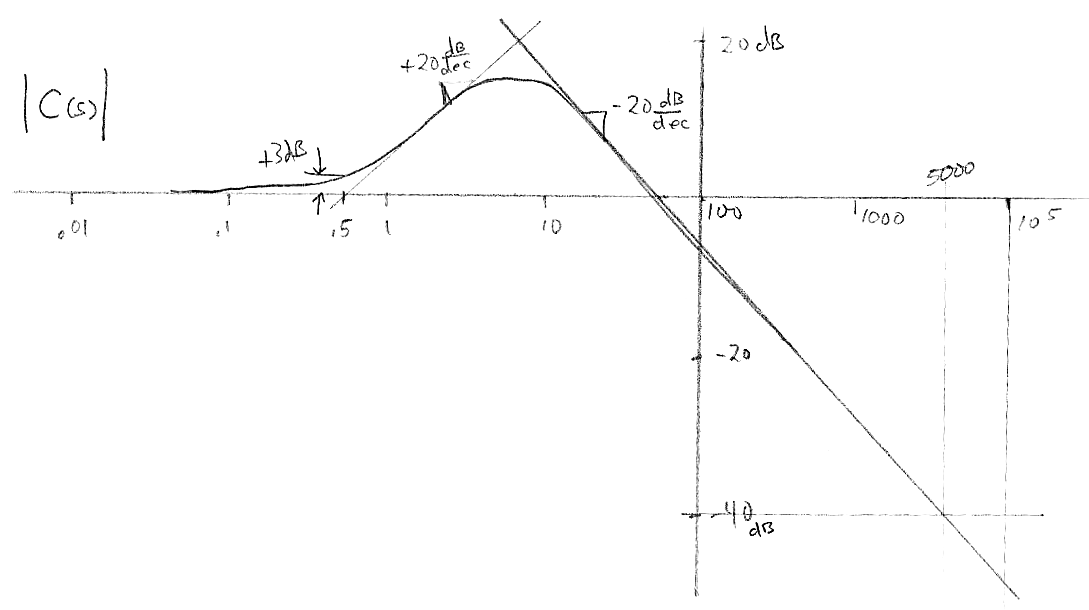
\includegraphics[width=3.5in]{figs11/01118.png}

We can see that the curve intersects $-40dB$ at $\omega_b=5000$.   Thus
\[
f_{samp} = 2\times\omega_b =  10,000 rad/sec = 1592 Hz
\]
\end{ExampleSmall}


%\end{frame}
\section{Digital Control Systems}


\begin{figure}\centering
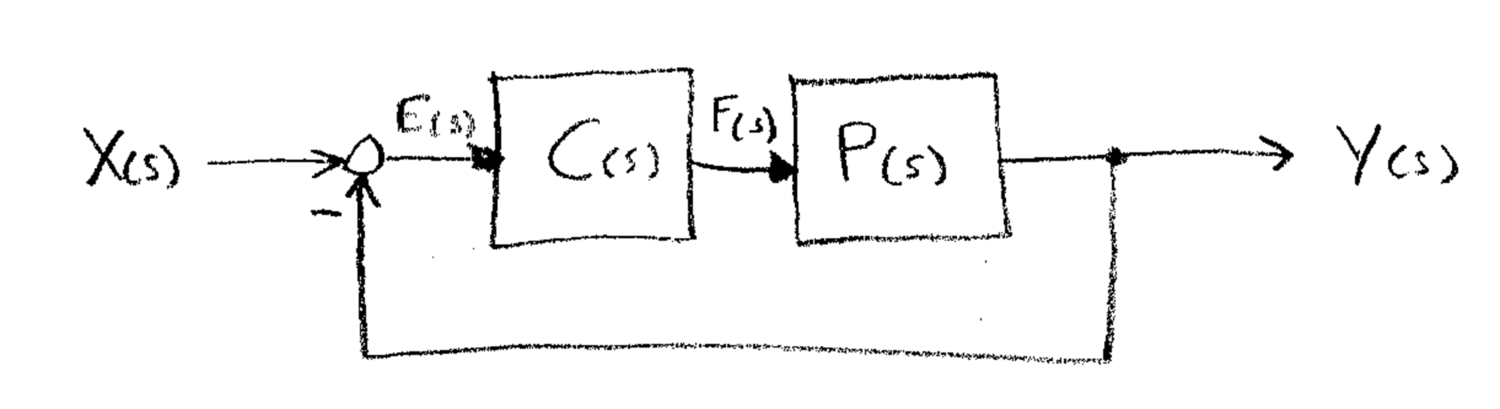
\includegraphics[width=5.0in]{figs11/ct_cl_sysa.png}
\caption{Closed loop continuous time control system.  Assume that we have designed a transfer function $C(s)$ which gives us a satisfactory system response.}\label{F:ct_cl}
\end{figure}
%\end{frame}

\begin{figure}\centering
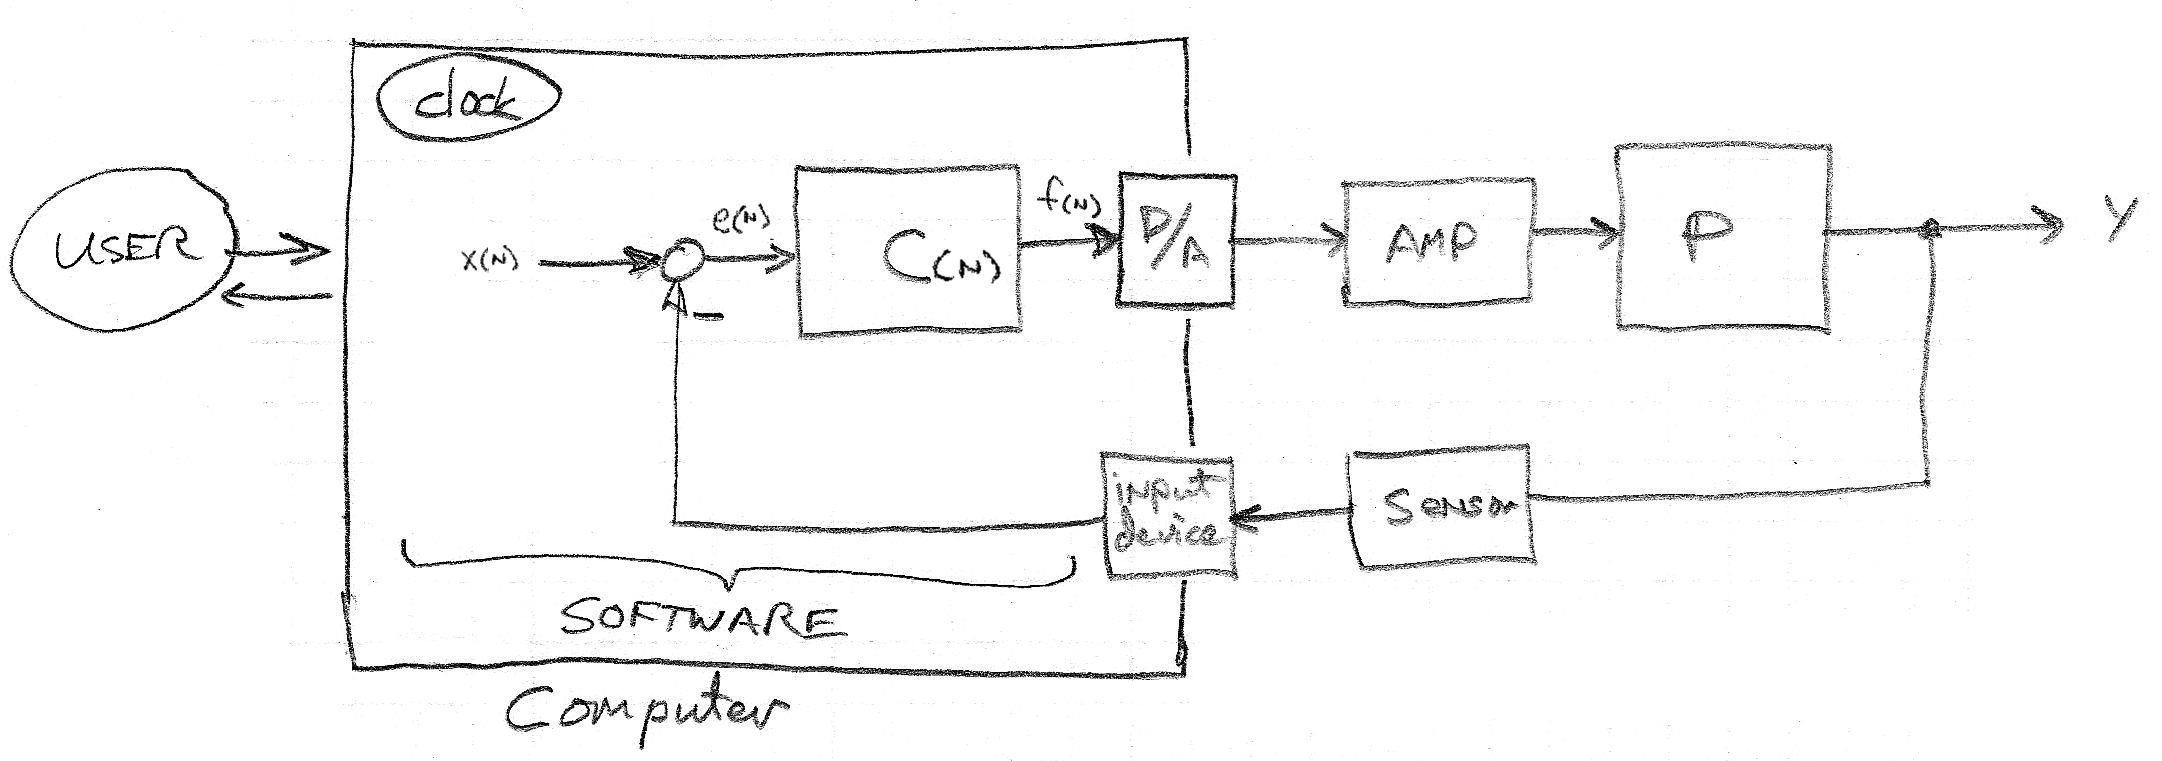
\includegraphics[width=6.00in]{figs11/01106.png}
\caption{Closed loop   control system using a computer, a digital-to-analog (D/A) converter, an amplifier (AMP) to increase power output to the plant (P) and a sensor for feedback to the controller.  $C$ refers to a discrete time implementation, $C(n)$ of $C(t)$.}\label{F:dt_cl}
\end{figure}



Let's put these ideas to work on  a control system such as that of Figure \ref{F:ct_cl}.
We want to implement the control system in a computer.
The plant, $P(s)$, of course stays outside the computer system since it is NOT a simulation.
A control system implemented by computer would thus look like the parts of Figure \ref{F:dt_cl} which are inside the box.
Refering to  Figure \ref{F:dt_cl}, an input $x(n)$  is provided, for example from a user interface.  The actual system output is sensed by a sensor  and sampled (measured at regular points in time) by an input device, and error, $e(n)$, is computed in the computer.  The controller $C(n)$ is a digital filter creating the force output, $f(n)$, which is applied to the plant by a digital-to-analog converter plus amplifier.


%%%%** Section 3
\section{Tustin's Method}
%\begin{frame}
%\frametitle{Tustin's Method}

Suppose we have a continuous time system (i.e. a Laplace Transform transfer function), $H(s)$.   Arnold Tustin developed
the following way to derive a Z-transform transfer function which is a digital approximation
to $H(s)$:
\[
H(z) = H(s)|_{s=\frac{2(z-1)}{T(z+1)}}
\]
Where $T$ is the sampling time.
In words,  to generate a discrete version of $H(s)$,  substitute ${\frac{2(z-1)}{T(z+1)}}$ for $s$ in $H(s)$.


%\end{frame}
%%%%** Section 3.1
\subsection{Tustin's method examples}
%\begin{frame}
%\frametitle{Example 1}

\begin{Example}	%<h>

Apply Tustin's method to convert $C(s)$ into $G(z)$ for $T$=1 sec. where
\[
C(s) = \frac{F(s)}{E(s)} = \frac{50}{(s+10)}
\]


%\end{frame}
%\begin{frame}
%\frametitle{Answer:}

Applying Tustin's method, plug in $\frac{2(z-1)}{T(z+1)}$ for $s$:
\[
C(z) = \frac{F(z)}{E(z)} = \frac{50}{(\frac{2(z-1)}{T(z+1)}+10)}
\]
\[
C(z) = \frac{50T(z+1)}              {2(z-1)+10T(z+1)}
\]
Applying $T=1$,
\[
C(z) = \frac{50(z+1)}{2z-2+10z+10} = 50\frac{(z+1)}{12z+8}
\]
\[
C(z)  = \frac{50}{12}\frac{(z+1)}{(z+0.6667)}
\]
As with continuous time transfer functions, we get a ratio of polynomials (this time in $z$) and we want to normalize them.

{\bf Note:} For reasons we will see in Section \ref{Limitations}, $T=1$ would NOT be fast enough for this control system.
\end{Example}	%<h>



\begin{Example}
Apply Tustin's method to convert $G(s)$ into $G(z)$ for $T$=0.01 sec. where
\[
G(s) = \frac{10(s+4)}{(s+0.1)(s+100)}
\]
\[
G(s) = \frac{10(s+4)}{(s+0.1)(s+100)} = \frac{10(s+4)}{s^2+100.1s+10}
\]
\[
G(z) = \frac{10 (\frac{2(z-1)}{T(z+1)} + 4) }   {(\frac {2(z-1)} {T(z+1)})^2+100.1(\frac{2(z-1)}{T(z+1)}) + 10}
\]

 Let's multiply through by $T^2(z+1)^2$:	%<h>
\[
= \frac{10(2(z-1)T(z+1) + 4T^2(z+1)^2)}    {4(z^2-2z+1)+100.1(2(z-1)T(Z+1))+10T^2(z+1)^2}
\]

Here's a couple of intermediate results we can plug in twice below:	%<h>
\[
2(z-1)T(z+1) = 0.02(z^2-1)  \qquad   T^2(z+1)^2 = 10^{-4}(z^2+2z+1)
\]

\[
G(z) = \frac   {10(0.02(z^2-1) + 4\times10^{-4}(z^2+2z+1))}          {4z^2-8z+4+2.02(z^2-1)+10^{-3}(z^2+2z+1)}
\]
\[
= \frac   {0.204z^2+0.008z-0.1960}        {6.021z^2-8.002z+1.981}
\]
\[
G(z) = 0.339 \frac   {z^2+0.03922z -0.9608}      {z^2-1.3290z+0.3290}
\]
{\bf Note:} For reasons we will see in Section \ref{Limitations}, $T=0.01$ would NOT be fast enough for this control system.
\end{Example}	%<h>


%\end{frame}

\subsection{Conversion  by  Computer}

In {\tt python.control} there is a built in function to convert transfer functions
from continuous time to discrete time, {\tt control.sample\_system()}.


\begin{listing}
\begin{minted}{python}
  import numpy as np
  import control as ctl
  s = ctl.TransferFunction.s
  # orig continuous time system
  sysCT = 20*(s+1)/((s+0.01)*(s+0.20)*(s+10))
  #  Now set up conversion (2 examples)
  fs = 20  # 2x highest pole/zero sampling
  Ts = 1/fs  # Sample time
  sysDT01 = ctl.sample_system(sysCT, Ts, method='tustin')
  fs = 40  # 4x highest pole/zero sampling
  Ts = 1/fs  # Sample time
  sysDT02 = ctl.sample_system(sysCT, Ts, method='tustin')
  print('\n          ECE 447 Example: Conversion to Discrete Time: \n')
  print('Continuous Time System: ',sysCT)
  print('\nDiscrete Time System (20Hz): ',  sysDT01 )
  print('\nDiscrete Time System (40Hz): ',  sysDT02 )
\end{minted}
\caption{Conversion to discrete time system using two different sampling times ({\tt Ts}).}
\label{lst:basicTustin}
\end{listing}


\begin{Example}
Convert the continuous time system $G(s)$ to discrete time.

% 20*(s+1)/((s+0.01)*(s+0.20)*(s+10))
 \[
 G(s) = \frac {20(s+1)}  {(s+0.01)(s+0.2)(s+10)}
 \]
We have very limited computing power available due to a low target for system cost.
Compute two versions of a discrete time system, for two sample times:
\[
T_1 = 2\times {\mathrm the highest pole or zero.}
\]
\[
T_1 = 4\times {\mathrm the highest pole or zero.}
\]

Code for this is given in Listing \ref{lst:basicTustin}.   Output is
\begin{verbatim}
                ECE 447 Example: Conversion to Discrete Time:

  Continuous Time System:  <TransferFunction>: sys[12]
  Inputs (1): ['u[0]']
  Outputs (1): ['y[0]']

  20 s + 20
  --------------------------------
  s^3 + 10.21 s^2 + 2.102 s + 0.02

  Discrete Time System (20Hz):  <TransferFunction>: sys[12]$sampled
  Inputs (1): ['u[0]']
  Outputs (1): ['y[0]']

  0.0102 z^3 + 0.01069 z^2 - 0.009202 z - 0.009699
  ------------------------------------------------
  z^3 - 2.59 z^2 + 2.183 z - 0.5937
  dt = 0.05

  Discrete Time System (40Hz):  <TransferFunction>: sys[12]$sampled
  Inputs (1): ['u[0]']
  Outputs (1): ['y[0]']

  0.002805 z^3 + 0.002874 z^2 - 0.002667 z - 0.002736
  ---------------------------------------------------
  z^3 - 2.773 z^2 + 2.546 z - 0.7737
  dt = 0.025
\end{verbatim}
\end{Example}


%\begin{frame}[containsverbatim]

% {\bf SCILAB }
%
% In  Scilab we will apply  Tustin's method more  directly:
% %\end{frame}

% %\begin{frame}[containsverbatim]
%
% \begin{verbatim}
%
% -->T = 0.01;
%
% -->m =  (2/T)*(z-1)/(z+1)
%  m  =
%
%   - 200 + 200z
%     ----------
%       1 + z
%
% -->pz = 10*(m+4)/((m+0.1)*(m+100))
%  pz  =
%
%                                        2
%   - 0.0326503 + 0.0013327z + 0.0339830z
%     -----------------------------------
%                                   2
%         0.3330002 - 1.3323338z + z
%
% \end{verbatim}
%
%
%  {\bf MATLAB}	%<hn>
%
%  Matlab has a function called {\tt c2d()} which converts continuous to discrete time systems.  It has multiple methods it can use but one of them is Tustin's. The arguments to the c2d function are:  the system, $T$, and the name of the method in string form:	%<hn>
%
% {\bf Matlab computation: }
% \begin{verbatim}
% >> g
%
% Zero/pole/gain:
%    10 (s+4)
% ---------------
% (s+0.1) (s+100)
%
% >> sz = c2d(g,0.01,'tustin')
%
% Zero/pole/gain:
% 0.033983 (z-0.9608) (z+1)
% -------------------------
%   (z-0.999) (z-0.3333)
%
% Sampling time: 0.01
% >>
% \end{verbatim}
% %\end{frame}
%
%
% %\begin{frame}[containsverbatim]
%
% You can  verify  that  this result is the same as Scilab's.

%\end{frame}

	%<*h>
Note that in this type of computation we should NOT round our results.  An exact rule for how
much precision we need in the coefficients of the digital filter is beyond the scope of the
course.  However you should use at least 6 digits in the problems we will work on.

Now that we have our controller in Z-transform form, we need one more step before we can code it: we need to convert it to a digital filter.
	%<*>

%%%%** Section 3.3
\subsection{Conversion of discrete transfer function to digital filter}
%\begin{frame}
%\frametitle{Conversion of discrete transfer function to digital filter}

First, we ``unwrap'' the transfer function so that it is now the Z transform of a digital filter.  Unwrapping is actually a simple step.  For example, using our first example above,
\[
C(z) = \frac{F(z)}{E(z)} = \frac{50}{12}\frac{(z+1)}{(z+0.6667)}
\]
we just cross multiply by the two denominators to get
\[
F(z) (z+0.6667) = \frac{50}{12} E(z) (z+1)
\]
or
\[
zF(z)+0.6667F(z) = 4.1667 (z E(z) + E(z))
\]

%\end{frame}
%\begin{frame}

Now, there is an important property of the Z-transform:	%<h>
% Z Transform delay property:
\[
Z\{x[n-k]\} = z^{-k}X(z)
\]
 In  words, shifting a signal in the time domain by $k$ samples is equivalent to multiplying by $z^{-k}$ in the Z domain.   Looking at it another way, we have a transform pair:	%<h>
% or ...
\[
x[n+k] \leftrightarrow z^{k}X(z)
\]

%\end{frame}
%\begin{frame}
Returning to our example, and	%<h>
multiplying through by $z^{-1}$ will prove useful so we get:
\[
F(z)+0.6667z^{-1}F(z)) = 4.1667 ( E(z) + z^{-1}E(z))
\]
Applying the delay property  to our unwrapped transfer function  gives:	%<h>
%Applying delay property:
\[
f(n)+0.6667f(n-1) = 4.1667 (e(n) + e(n-1))
\]

%\end{frame}
%\begin{frame}
%%%%** Figure 3
\begin{figure}\centering
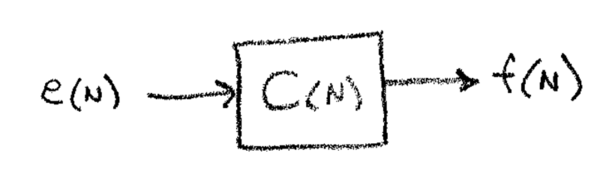
\includegraphics[width=2.0in]{figs11/dt_ctlra.png}
\caption{Just the controller part of the system.}\label{F:dt_ctl}
\end{figure}

Let's step back a bit and recall that our controller is a relationship between the sampled error in our control system ($e(n)$) and the sampled controller output ($f(n)$, Figure \ref{F:dt_ctl}).  Isolating $f(n)$,	%<h>
\[
f(n) = 4.1667 (e(n) + e(n-1))-0.6667f(n-1)
\]

This is essentially the line of computer code which defines our controller!  	%<h>

%\end{frame}
%\begin{frame}
%\frametitle{Implementation Block Diagram}

 We could implement this equation with the block diagram of Figure \ref{F:DigitalControl}.	%<h>

%%%%** Figure 4
\begin{figure}\centering
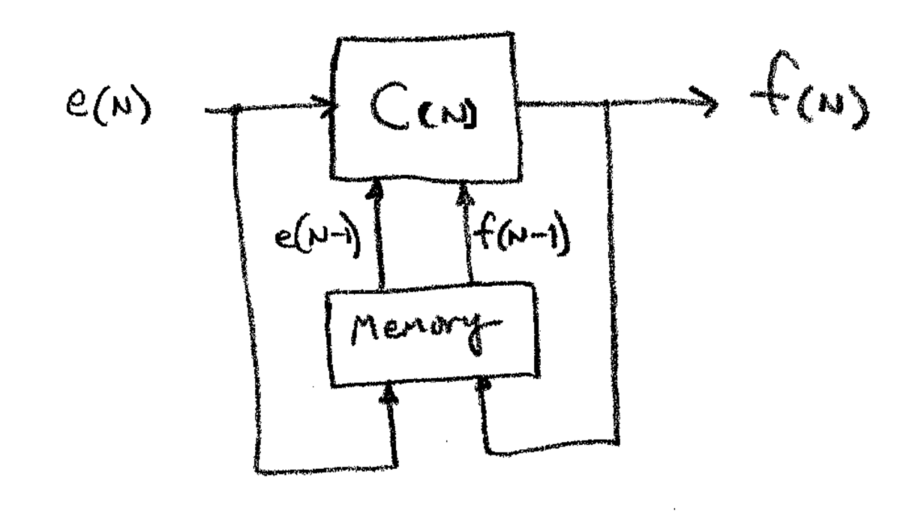
\includegraphics[width=3.0in]{figs11/dig_ctl_bda.png}
\caption{A way to implement the example digital controller.  The memory stores previous values for $e(n), f(n)$. }\label{F:DigitalControl}
\end{figure}


%\end{frame}

%%%%** Section 4
\section{Code Example}

 Let's put this equation into some computer code.  We will not worry about many details such as the operating system or exact computer syntax, and we will assume that functions are available to do the I/O for us.


\begin{listing}
\begin{minted}{C}
/*  EE447, U. of Washington.  Example of basic digital control code  */
double e, x, f;    // define our system loop variables
double ys;         // this will be our sensed y for feedback
double en1, fn1;   //  these will be e(n-1) etc.
int T=1000;      // sampling time in milli seconds.
int t, t1;      // variables for keeping track of time.
en1 = fn1 = 0.0;   // we have to start them with something!
// loop forever
while(1)  {
  t = get_current_time();
  x = get_command_input();  // get our input from somewhere
  ys = read_sensor();       // get feedback from our system
  en  = x-ys;                // compute error (H=1)

  f = 4.1667 * (en+en1) - 0.6667*fn1;   // compute controller output

  output_to_plant(f);       // send controller output to plant
  en1 = en;                  // store previous values of e, f
  fn1 = f;
  t1 = get_current_time();
  wait(T-(t-t1));           // wait for next sample time
  }
\end{minted}
\caption{Example of a pseudocode application which implements a discrete time controller.}
\label{lst:DigitalControlLoop}
\end{listing}	%<*>

%\end{frame}

	%<*h>
The code runs (Listing \ref{lst:DigitalControlLoop}) in an infinite loop (line 10) and executes the controller over and over.  First, we note the current time and store it in {\tt t}.  We get the controller input, for example from a user interface or a trajectory generator, in line 12.   Then we read a sensor to measure the actual output {\tt ys} (line 13).  After we compute the error, we are ready to compute the controller output (line 16) using the equation we derived above.  Note that the coefficients in line 16 are specific to $T=1.0$ and will be wrong if we arbitrarily change {\tt T} in the code.   After we put the controller output out to the plant (line 18) we store the current values of {\tt e, f} in the previous values for use in the next cycle.   Finally, we figure out how much time has elapsed between lines 11 and 23, and use that to derive the correct argument for a {\tt wait(t)} function so that our timing is accurate.
	%<*>

%%%%** Section 5
\section{Limitations and properties}\label{Limitations}
%\begin{frame}
%\frametitle{Limitations and Properties}
 Tustin's method creates a controller which only approximates the continuous time controller. However useful discrete time controllers can be made if the following properties and limitations are taken into account.	%<h>

\begin{itemize}
  \item If the continous time TF is stable then the discrete time version will be stable.
  \item The DT controller will have the same ``features''  of its frequency response (number and frequency order of poles and zeros) as the CT controller.
  \item Frequencies of the poles and zeros will in general be shifted.
  \item For frequencies much less than the Nyquist rate ($f_N$), the approximation will be very accurate.
\end{itemize}


%\end{frame}
%\begin{frame}
To make sure the discrete time controller is accurate, make sure that $T<<\pi/pz$ where $pz$ is the frequency of the highest pole or zero in the CT system (including both $C(s)$ and $P(s)$).   For example, let
\[
C_1(s) = \frac{500(s+10)}{(s+1)(s+100)}
\]
For this controller, $pz = 100rad/sec$.   This is about 16$Hz$.
We need to double this to account for Nyquist sampling and THEN multiply by 10 to make the frequencies of the poles ``much less'' than the Nyquist rate.

Thus a suitable sampling frequency would be $16\times2\times10 = 320$ samples/second.  We would convert $C_1(s)$ to discrete time using $T=0.003125 = 1/320 sec$).



% \section{Summary of Notation}

